\documentclass{article}\usepackage[]{graphicx}\usepackage{xcolor}
%% maxwidth is the original width if it is less than linewidth
%% otherwise use linewidth (to make sure the graphics do not exceed the margin)
\makeatletter
\def\maxwidth{ %
  \ifdim\Gin@nat@width>\linewidth
    \linewidth
  \else
    \Gin@nat@width
  \fi
}
\makeatother

\definecolor{fgcolor}{rgb}{0.345, 0.345, 0.345}
\newcommand{\hlnum}[1]{\textcolor[rgb]{0.686,0.059,0.569}{#1}}%
\newcommand{\hlstr}[1]{\textcolor[rgb]{0.192,0.494,0.8}{#1}}%
\newcommand{\hlcom}[1]{\textcolor[rgb]{0.678,0.584,0.686}{\textit{#1}}}%
\newcommand{\hlopt}[1]{\textcolor[rgb]{0,0,0}{#1}}%
\newcommand{\hlstd}[1]{\textcolor[rgb]{0.345,0.345,0.345}{#1}}%
\newcommand{\hlkwa}[1]{\textcolor[rgb]{0.161,0.373,0.58}{\textbf{#1}}}%
\newcommand{\hlkwb}[1]{\textcolor[rgb]{0.69,0.353,0.396}{#1}}%
\newcommand{\hlkwc}[1]{\textcolor[rgb]{0.333,0.667,0.333}{#1}}%
\newcommand{\hlkwd}[1]{\textcolor[rgb]{0.737,0.353,0.396}{\textbf{#1}}}%

\usepackage{framed}
\makeatletter
\newenvironment{kframe}{%
 \def\at@end@of@kframe{}%
 \ifinner\ifhmode%
  \def\at@end@of@kframe{\end{minipage}}%
  \begin{minipage}{\columnwidth}%
 \fi\fi%
 \def\FrameCommand##1{\hskip\@totalleftmargin \hskip-\fboxsep
 \colorbox{shadecolor}{##1}\hskip-\fboxsep
     % There is no \\@totalrightmargin, so:
     \hskip-\linewidth \hskip-\@totalleftmargin \hskip\columnwidth}%
 \MakeFramed {\advance\hsize-\width
   \@totalleftmargin\z@ \linewidth\hsize
   \@setminipage}}%
 {\par\unskip\endMakeFramed%
 \at@end@of@kframe}
\makeatother

\definecolor{shadecolor}{rgb}{.97, .97, .97}
\definecolor{messagecolor}{rgb}{0, 0, 0}
\definecolor{warningcolor}{rgb}{1, 0, 1}
\definecolor{errorcolor}{rgb}{1, 0, 0}
\newenvironment{knitrout}{}{} % an empty environment to be redefined in TeX

\usepackage{alltt}
\IfFileExists{upquote.sty}{\usepackage{upquote}}{}
\begin{document}

\section*{Additional files}

  In the main text of this manuscript, we showed the fitting and simulating results for Cat 1. Here, we have the adjusted BIC emission distribution comparisons, adjusted BIC across all FMM and HMM models, diurnal step lengths and autocorrelation plots for Cat 2, 14, and 15. Given we have not account for sex, we can see in that our fitting and predictions are better for male cats (Cat 1 and 2) than female cats (Cat 14, 15). 
  
\newpage


















\begin{knitrout}
\definecolor{shadecolor}{rgb}{0.969, 0.969, 0.969}\color{fgcolor}\begin{figure}
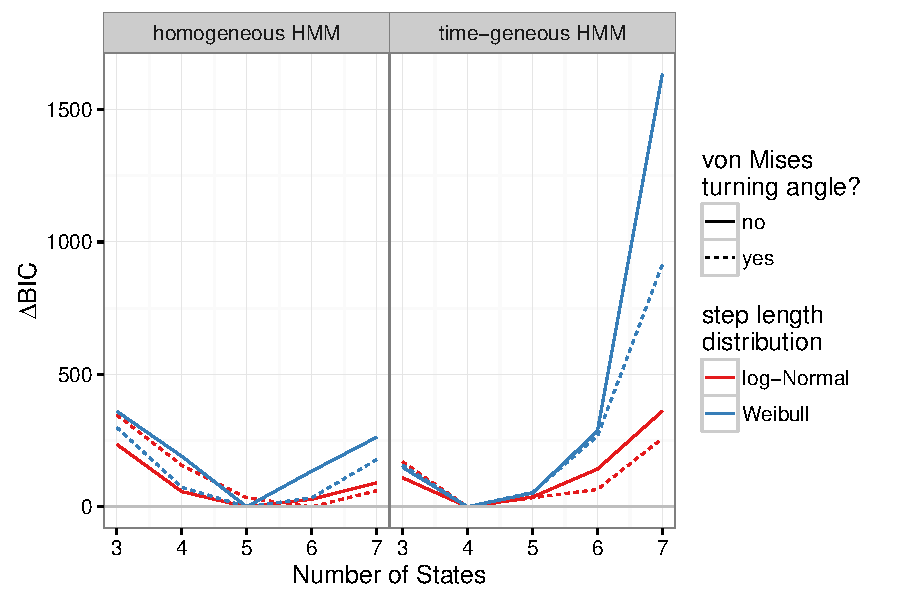
\includegraphics[width=\maxwidth]{figure/BICred_plot2-1} \caption[Adjusted BIC Emission Distribution Comparison for Cat 2]{Adjusted BIC Emission Distribution Comparison for Cat 2}\label{fig:BICred_plot2}
\end{figure}


\end{knitrout}

\clearpage
\begin{knitrout}
\definecolor{shadecolor}{rgb}{0.969, 0.969, 0.969}\color{fgcolor}\begin{figure}
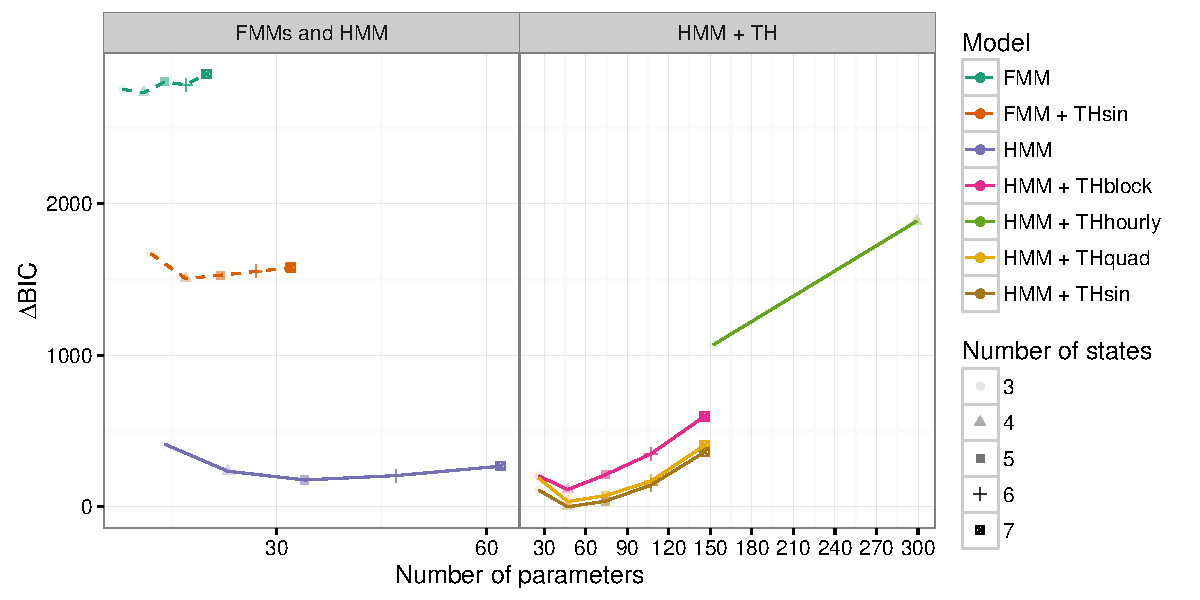
\includegraphics[width=\maxwidth]{figure/adj_BIC_comparisons2-1} \caption[Adjusted BICs Across All Models for Cat 2]{Adjusted BICs Across All Models for Cat 2}\label{fig:adj_BIC_comparisons2}
\end{figure}


\end{knitrout}

\clearpage

\begin{knitrout}
\definecolor{shadecolor}{rgb}{0.969, 0.969, 0.969}\color{fgcolor}\begin{figure}
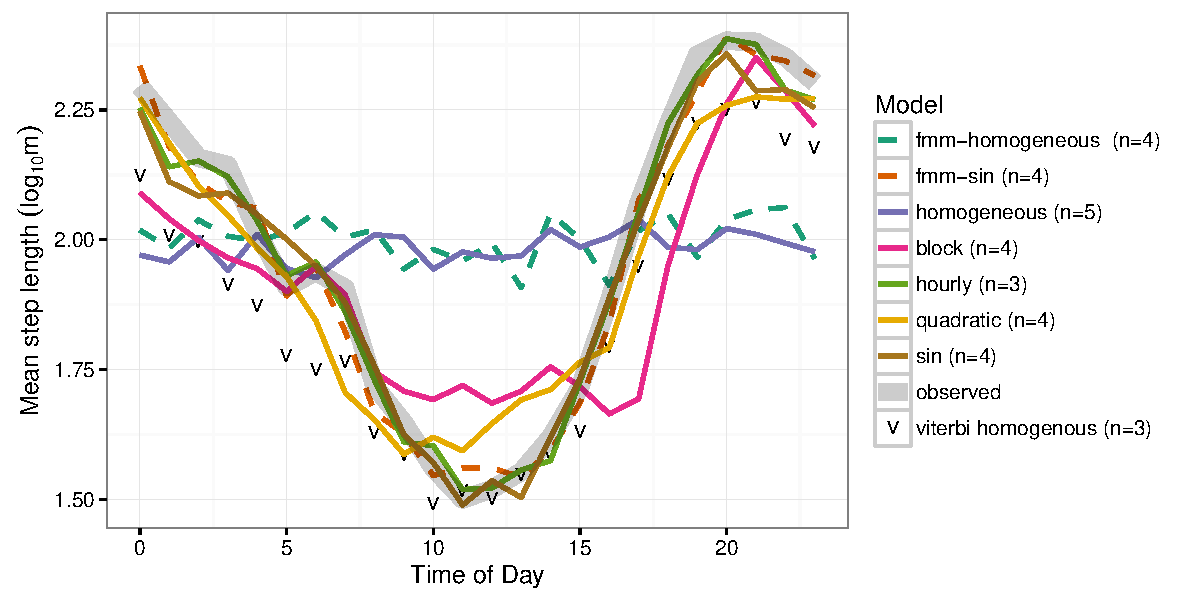
\includegraphics[width=\maxwidth]{figure/avg_step_length_by_time2-1} \caption[Diurnal Step Lengths Plot for Cat 2]{Diurnal Step Lengths Plot for Cat 2}\label{fig:avg_step_length_by_time2}
\end{figure}


\end{knitrout}

\clearpage

\begin{knitrout}
\definecolor{shadecolor}{rgb}{0.969, 0.969, 0.969}\color{fgcolor}\begin{figure}
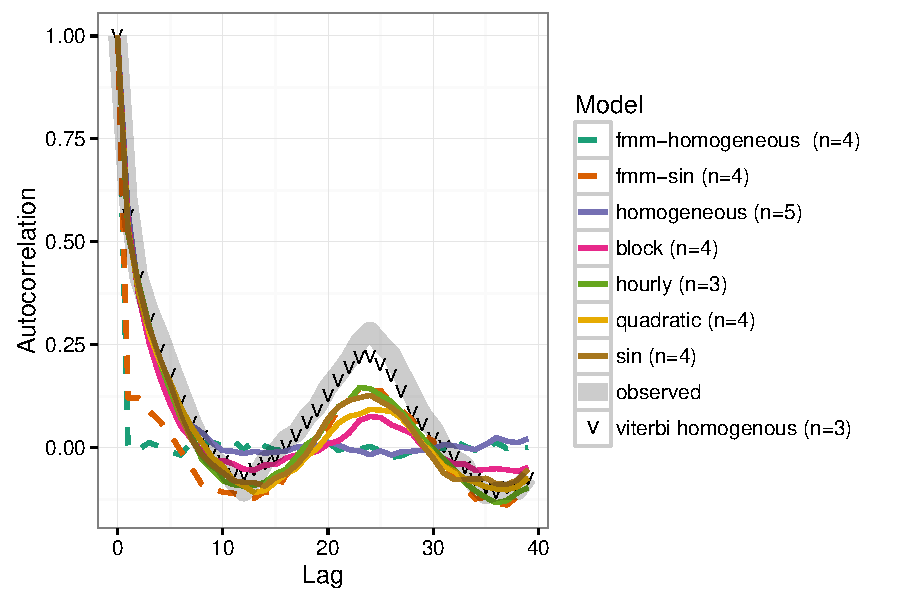
\includegraphics[width=\maxwidth]{figure/acf_plot2-1} \caption[Autocorrelation Plot for Cat 2]{Autocorrelation Plot for Cat 2}\label{fig:acf_plot2}
\end{figure}


\end{knitrout}


\clearpage
%cat14

\begin{knitrout}
\definecolor{shadecolor}{rgb}{0.969, 0.969, 0.969}\color{fgcolor}\begin{figure}
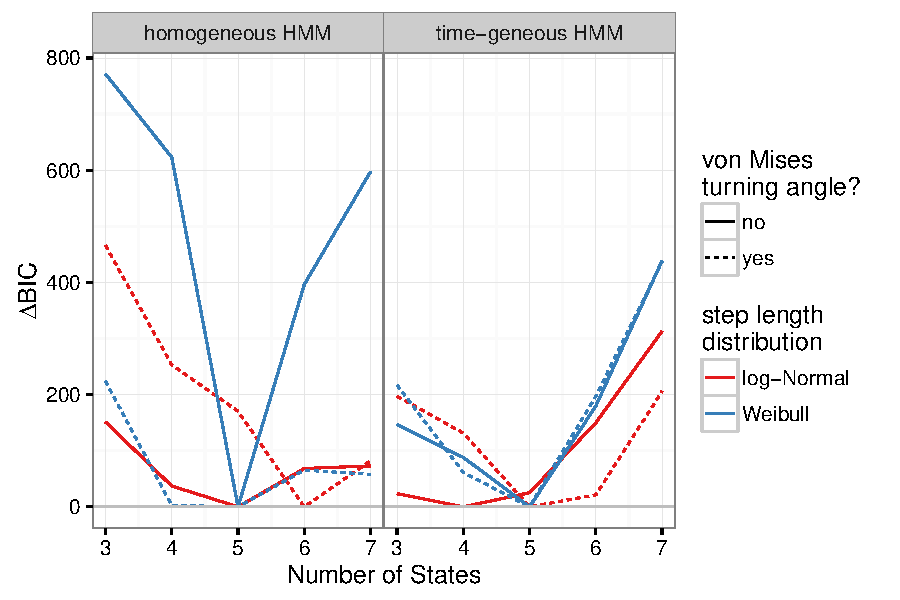
\includegraphics[width=\maxwidth]{figure/BICred_plot14-1} \caption[Adjusted BIC Emission Distribution Comparison for Cat 14]{Adjusted BIC Emission Distribution Comparison for Cat 14}\label{fig:BICred_plot14}
\end{figure}


\end{knitrout}


\clearpage

\begin{knitrout}
\definecolor{shadecolor}{rgb}{0.969, 0.969, 0.969}\color{fgcolor}\begin{figure}
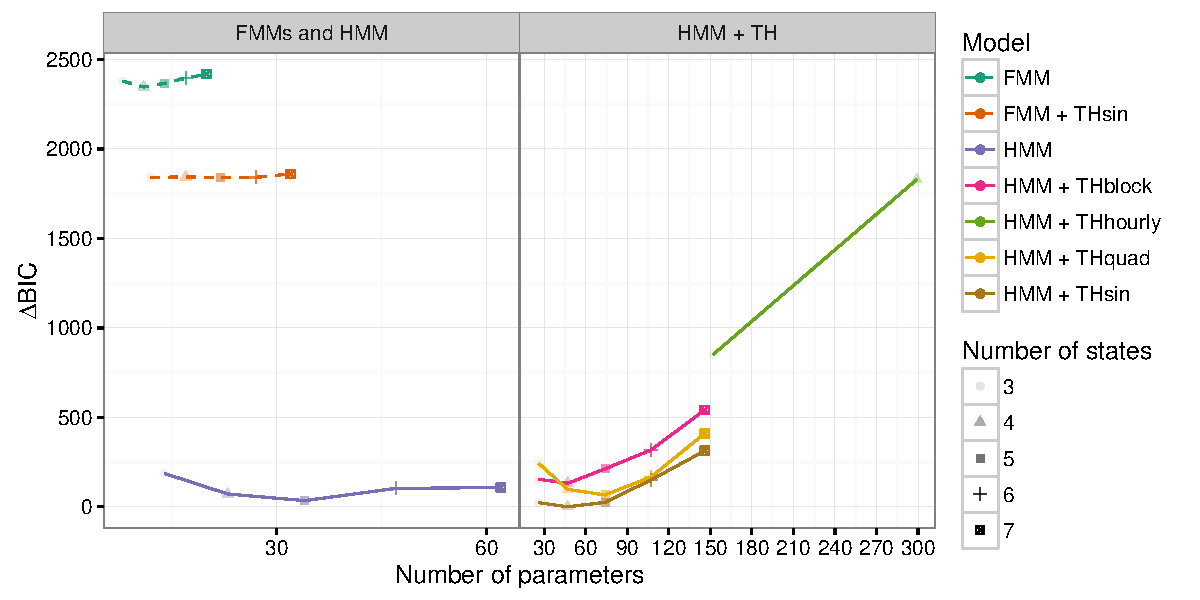
\includegraphics[width=\maxwidth]{figure/adj_BIC_comparisons14-1} \caption[Adjusted BICs Across All Models for Cat 14]{Adjusted BICs Across All Models for Cat 14}\label{fig:adj_BIC_comparisons14}
\end{figure}


\end{knitrout}

\clearpage

\begin{knitrout}
\definecolor{shadecolor}{rgb}{0.969, 0.969, 0.969}\color{fgcolor}\begin{figure}
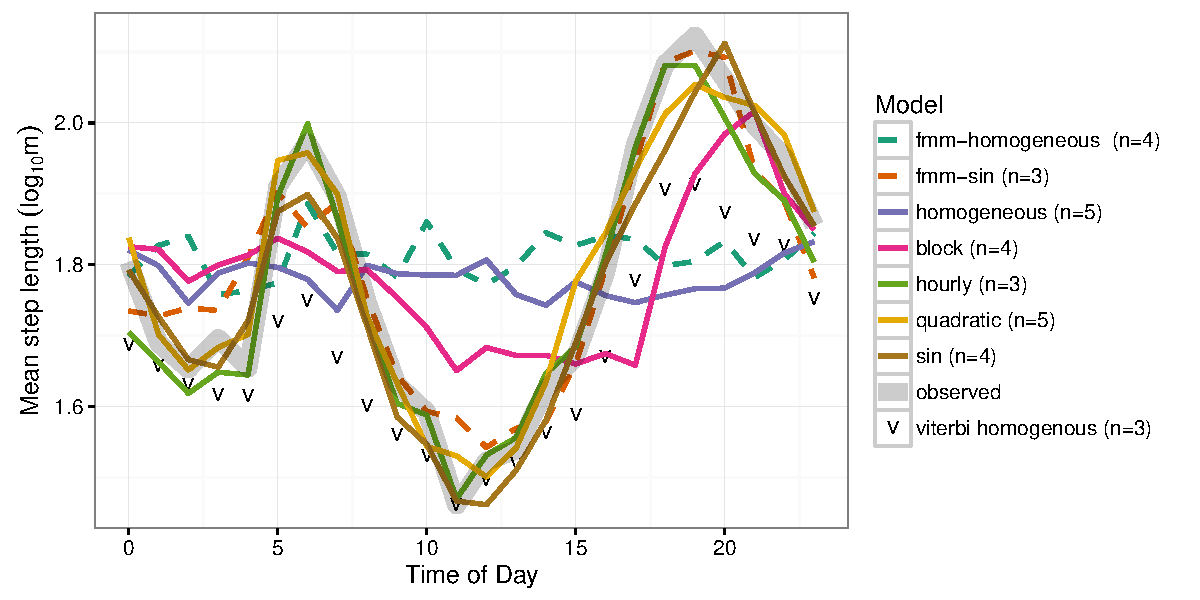
\includegraphics[width=\maxwidth]{figure/avg_step_length_by_time14-1} \caption[Diurnal Step Lengths Plot for Cat 14]{Diurnal Step Lengths Plot for Cat 14}\label{fig:avg_step_length_by_time14}
\end{figure}


\end{knitrout}

\clearpage

\begin{knitrout}
\definecolor{shadecolor}{rgb}{0.969, 0.969, 0.969}\color{fgcolor}\begin{figure}
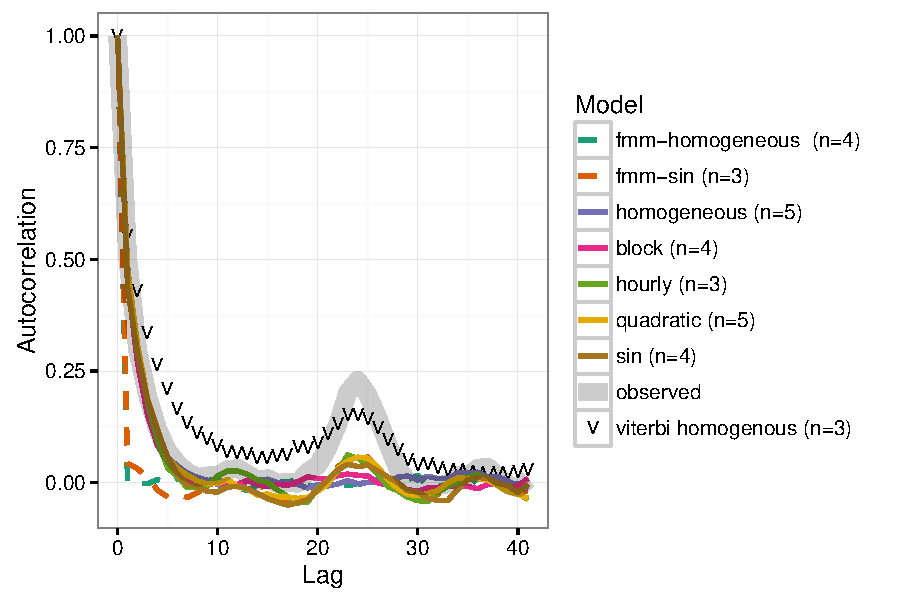
\includegraphics[width=\maxwidth]{figure/acf_plot14-1} \caption[Autocorrelation Plot for Cat 14]{Autocorrelation Plot for Cat 14}\label{fig:acf_plot14}
\end{figure}


\end{knitrout}

\clearpage
%cat15

\begin{knitrout}
\definecolor{shadecolor}{rgb}{0.969, 0.969, 0.969}\color{fgcolor}\begin{figure}
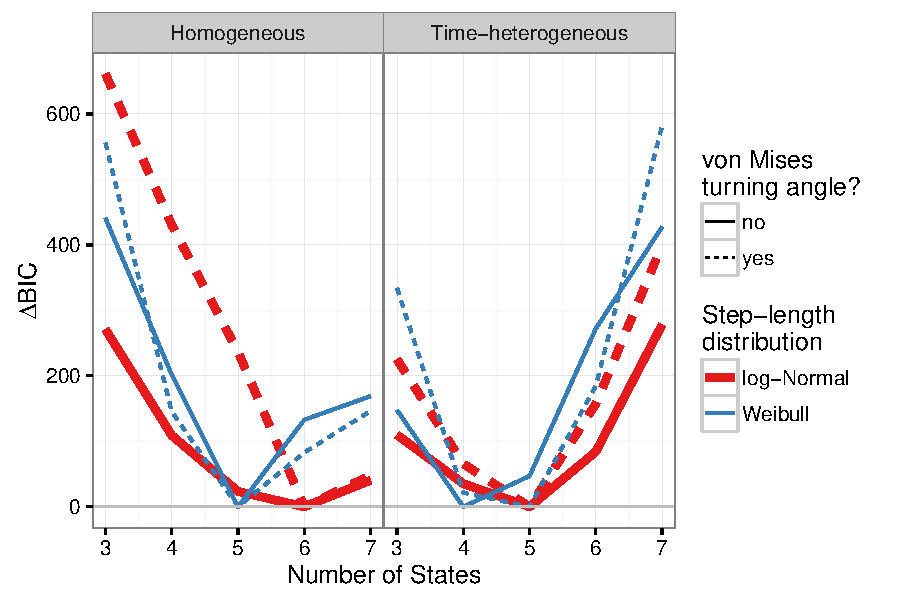
\includegraphics[width=\maxwidth]{figure/BICred_plot15-1} \caption[Adjusted BIC Emission Distribution Comparison for Cat 15]{Adjusted BIC Emission Distribution Comparison for Cat 15}\label{fig:BICred_plot15}
\end{figure}


\end{knitrout}


\clearpage

\begin{knitrout}
\definecolor{shadecolor}{rgb}{0.969, 0.969, 0.969}\color{fgcolor}\begin{figure}
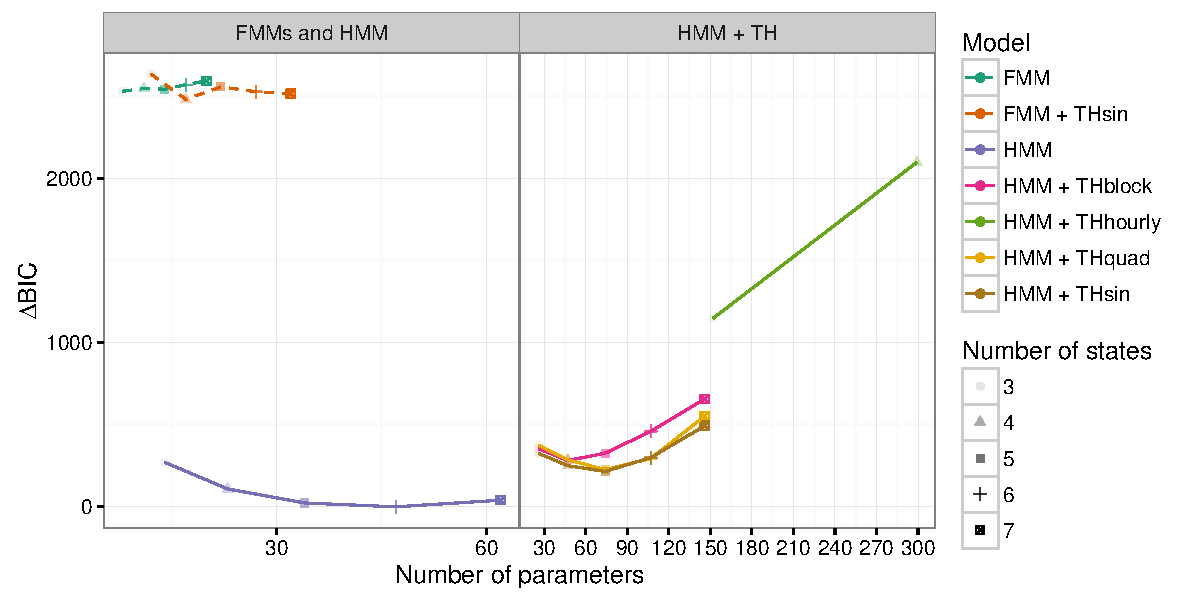
\includegraphics[width=\maxwidth]{figure/adj_BIC_comparisons15-1} \caption[Adjusted BICs Across All Models for Cat 15]{Adjusted BICs Across All Models for Cat 15}\label{fig:adj_BIC_comparisons15}
\end{figure}


\end{knitrout}

\clearpage

\begin{knitrout}
\definecolor{shadecolor}{rgb}{0.969, 0.969, 0.969}\color{fgcolor}\begin{figure}
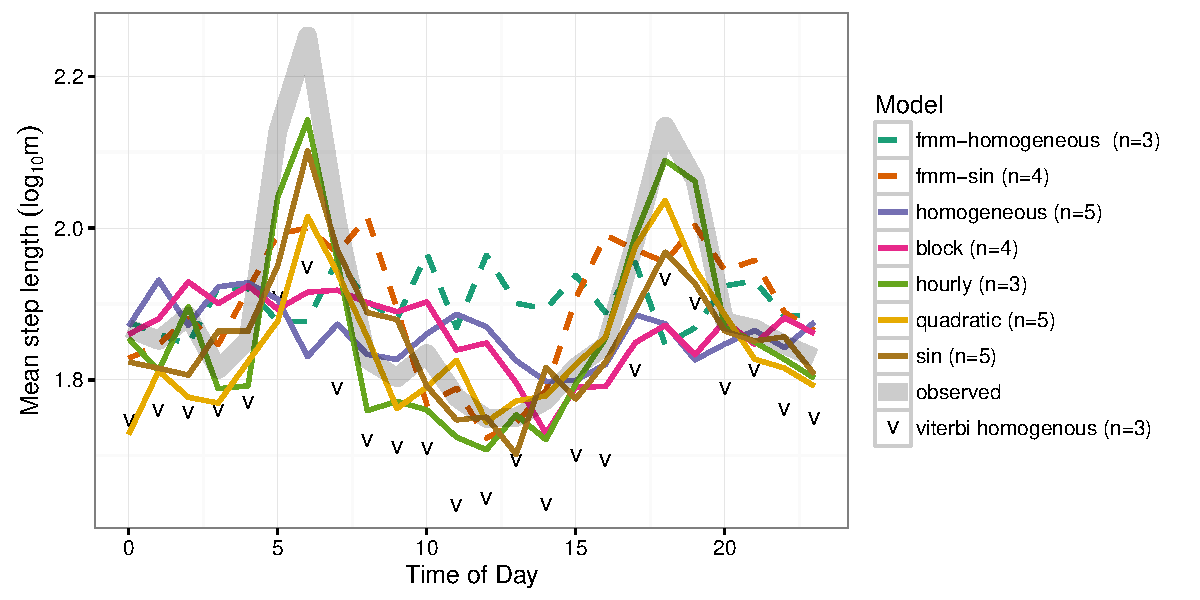
\includegraphics[width=\maxwidth]{figure/avg_step_length_by_time15-1} \caption[Diurnal Step Lengths Plot for Cat 15]{Diurnal Step Lengths Plot for Cat 15}\label{fig:avg_step_length_by_time15}
\end{figure}


\end{knitrout}

\clearpage

\begin{knitrout}
\definecolor{shadecolor}{rgb}{0.969, 0.969, 0.969}\color{fgcolor}\begin{figure}
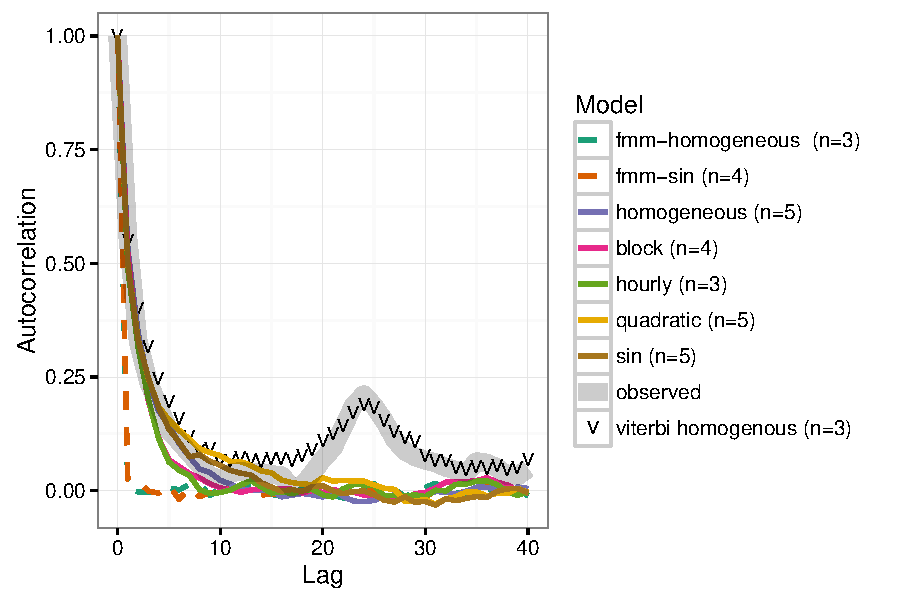
\includegraphics[width=\maxwidth]{figure/acf_plot15-1} \caption[Autocorrelation Plot for Cat 15]{Autocorrelation Plot for Cat 15}\label{fig:acf_plot15}
\end{figure}


\end{knitrout}

\end{document}
